% **************************************************
% Author:Jiankun WANG
% **************************************************

% **************************************************
% !!! Read Me !!!
% (1)Use Texstudio 
% (2)click Options-->Configure TexStudio-->Builder-->Default Complier:XeLatex
% (3)click Options-->Configure TexStudio-->Builder-->Default Bibliography:Biber
% (4)Encoding:UTF-8
% (5)if something wrong in bibliography, click Tools-->Command-->Biber
% (6)Compile the Chinese abstract with package xeCJK before the final version,
%    since compling xeCJK costs a long time
% **************************************************


% **************************************************
% Document Class Definition
% **************************************************
\documentclass[%
    paper=A4,               % paper size --> A4 is default in Germany
    twoside=true,           % onesite or twoside printing
    openright,              % doublepage cleaning ends up right side
    parskip=full,           % spacing value / method for paragraphs
    chapterprefix=true,     % prefix for chapter marks
    12pt,                   % font size
    headings=normal,        % size of headings
    bibliography=totoc,     % include bib in toc
    listof=totoc,           % include listof entries in toc
    titlepage=on,           % own page for each title page
    captions=tableabove,    % display table captions above the float env
    draft=false,            % value for draft version
]{scrreprt}%

%\usepackage{xeCJK} % COMMENT THIS LINE BEFORE FINAL VERSION
\usepackage{graphics} % for pdf, bitmapped graphics files
\usepackage{graphicx}
\usepackage{subfigure}
\usepackage{rotating}%sidewaysfigure
\usepackage{booktabs}
\usepackage{multirow}
\usepackage{epsfig} % for postscript graphics files
\usepackage{times} % assumes new font selection scheme installed
\usepackage{amsmath} % assumes amsmath package installed
\usepackage{amssymb}  % assumes amsmath package installed
\usepackage{url}
\usepackage{epstopdf}
\usepackage{multicol}
\usepackage{bm}
\usepackage{mathrsfs}
\usepackage{color}
\usepackage[table]{xcolor}
\usepackage[T1]{fontenc}% optional T1 font encoding
\usepackage{float}
\usepackage{bigstrut}
\usepackage{balance}
\usepackage{caption}
\usepackage{amsopn}
\usepackage[linesnumbered,ruled,vlined]{algorithm2e}
\usepackage{placeins}
\usepackage{amsbsy}
\usepackage{amsthm}% for the lemma and proof
%\usepackage{CJKutf8}% for chinese
\newtheorem{lemma}{Lemma}
\newtheorem{mydef}{Definition}
\newtheorem{mythe}{Theorem}
\usepackage{url}

\usepackage[nottoc]{tocbibind}% automatically add the figure list and the table list to the content
\PassOptionsToPackage{subfigure}{tocloft} %Jiankun Changes to fix the bug

% **************************************************
% Setup YOUR thesis document in this file !
% **************************************************
% !TEX root = my-thesis.tex


% **************************************************
% Files' Character Encoding
% **************************************************
\PassOptionsToPackage{utf8}{inputenc}
\usepackage{inputenc}


% **************************************************
% Information and Commands for Reuse
% **************************************************
\newcommand{\thesisTitle}{An Adaptive Sampling-based Strategy for Mobile Robot Motion Planning}
\newcommand{\thesisName}{WANG, Jiankun}
\newcommand{\thesisSubject}{Documentation}
\newcommand{\thesisDate}{May 2019}
\newcommand{\thesisVersion}{My First Draft}

\newcommand{\thesisUniversity}{\protect{The Chinese University of Hong Kong}}
\newcommand{\thesisUniversityDepartment}{Electronic Engineering}
\newcommand{\thesisUniversityInstitute}{Institute for Clean Thesis Dev}
\newcommand{\thesisUniversityGroup}{Clean Thesis Group (CTG)}
\newcommand{\thesisUniversityCity}{Hong Kong}
\newcommand{\thesisUniversityStreetAddress}{Rm.432, Ho Sin-hang Engineering Buidling, The Chinese University of Hong Kong, Shatin, N.T.}
\newcommand{\thesisUniversityPostalCode}{Postal Code}


% **************************************************
% Debug LaTeX Information
% **************************************************
%\listfiles


% **************************************************
% Load and Configure Packages
% **************************************************
\usepackage[english]{babel} % babel system, adjust the language of the content
\PassOptionsToPackage{% setup clean thesis style
    figuresep=colon,%
    sansserif=false,%
    hangfigurecaption=false,%
    hangsection=true,%
    hangsubsection=true,%
    colorize=full,%
    colortheme=bluemagenta,%
    bibsys=biber,%
    bibfile=bib-refs,%
    bibstyle=numeric,%alphabetic,%
    wrapfooter=true,%false
}{cleanthesis}
\usepackage{cleanthesis}

\hypersetup{% setup the hyperref-package options
    pdftitle={\thesisTitle},    %   - title (PDF meta)
    pdfsubject={\thesisSubject},%   - subject (PDF meta)
    pdfauthor={\thesisName},    %   - author (PDF meta)
    plainpages=false,           %   -
    colorlinks=false,           %   - colorize links?
    pdfborder={0 0 0},          %   -
    breaklinks=true,            %   - allow line break inside links
    bookmarksnumbered=true,     %
    bookmarksopen=true          %
}



% **************************************************
% Document CONTENT
% **************************************************
\begin{document}

% --------------------------
% rename document parts
% --------------------------
\renewcaptionname{english}{\figurename}{Fig.}
\renewcaptionname{english}{\tablename}{Tab.}

% --------------------------
% Front matter
% --------------------------
\setstretch{1.2}
\pagenumbering{roman}			% roman page numbing (invisible for empty page style)
\pagestyle{empty}				% no header or footers
% !TEX root = ../index.tex
%
% By Tingting LIU
%
% ------------------------------------  --> cover title page
%\begin{titlepage}
%	\pdfbookmark[0]{Cover}{Cover}
%	\flushright
%	\hfill
%	\vfill
%	{\LARGE\thesisTitle \par}
%	\rule[5pt]{\textwidth}{.4pt} \par
%	{\Large\thesisName}
%	\vfill
%	\textit{\large\thesisDate} \\
%	%Version: \thesisVersion
%\end{titlepage}


% ------------------------------------  --> main title page
\begin{titlepage}
	%\pdfbookmark[0]{Titlepage}{Titlepage}
	\tgherosfont
	\centering
		
%	%{\Large \thesisUniversity} \\ [4mm]
%	\includegraphics[width=13cm]{pics/cuhk_logo.pdf} \\[5mm]
%	{\LARGE \textsf{\thesisUniversityDepartment}} \\ [5mm]
%	{\LARGE \textsf{\thesisUniversityInstitute}} \\
%	%\textsf{\thesisUniversityGroup} \\

	\vfill
	%\vspace*{2cm}
	%{\large \thesisSubject} \\[5mm]
	%{\LARGE \color{ctcolortitle}\textbf{\thesisTitle} \\[10mm]}
	%{\Large \thesisName} \\
	
	\vspace*{1.0cm}
    %{\LARGE \textbf{A Study of Dynamic Environment Perception Strategies using RGB-D Camera}} \\[15mm]
    {\LARGE \textbf{\thesisTitle} \\[30mm]}
	
	{\LARGE \thesisName } \\[30mm]
	{\Large A Thesis Submitted in Partial Fulfilment} \\[5mm]		
	{\Large of the Requirements for the Degree of} \\ [5mm]	
	{\Large Doctor of Philosophy} \\ [5mm]
	{\Large in } \\ [5mm]
	{\Large \thesisUniversityDepartment} \\  [40mm]
	{\Large \thesisUniversity} \\ [5mm]
 	{\Large \thesisDate}
 	
	
%	\vfill
%	\begin{minipage}[t]{.27\textwidth}
%		\raggedleft
%		\textit{1. Examiner}
%	\end{minipage}
%	\hspace*{15pt}
%	\begin{minipage}[t]{.65\textwidth}
%		{\Large \thesisFirstReviewer} \\
%	  	{\small \thesisFirstReviewerDepartment} \\[-1mm]
%		{\small \thesisFirstReviewerUniversity}
%	\end{minipage} \\[5mm]
%	
%	\begin{minipage}[t]{.27\textwidth}
%		\raggedleft
%		\textit{2. Examiner}
%	\end{minipage}
%	\hspace*{15pt}
%	\begin{minipage}[t]{.65\textwidth}
%		{\Large \thesisSecondReviewer} \\
%	  	{\small \thesisSecondReviewerDepartment} \\[-1mm]
%		{\small \thesisSecondReviewerUniversity}
%	\end{minipage} \\[5mm]
%	
%	\begin{minipage}[t]{.27\textwidth}
%		\raggedleft
%		\textit{3. Examiner}
%	\end{minipage}
%	\hspace*{15pt}
%	\begin{minipage}[t]{.65\textwidth}
%		{\Large \thesisThirdReviewer} \\
%	  	{\small \thesisThirdReviewerDepartment} \\[-1mm]
%		{\small \thesisThirdReviewerUniversity}
%	\end{minipage} \\[5mm]	
%	
%	\begin{minipage}[t]{.27\textwidth}
%		\raggedleft
%		\textit{Supervisor}
%	\end{minipage}
%	\hspace*{15pt}
%	\begin{minipage}[t]{.65\textwidth}
%		{\Large \thesisFirstSupervisor} %\ and \thesisSecondSupervisor
%	\end{minipage} \\[10mm]

%	\thesisDate \\

\end{titlepage}


% ------------------------------------  --> lower title back for single page layout
%\hfill
%\vfill
%{
%	\small
%	\textbf{\thesisName} \\
%	\textit{\thesisTitle} \\
%	%\thesisSubject,
%	\thesisDate \\
%	Examiners: \thesisFirstReviewer\ and \thesisSecondReviewer\ and \thesisThirdReviewer \\
%	Supervisor: \thesisFirstSupervisor \\[1.5em]
%	\textbf{\thesisUniversity} \\
%	%\textit{\thesisUniversityGroup} \\
%	\thesisUniversityInstitute \\
%	\thesisUniversityDepartment \\
%	\thesisUniversityStreetAddress \\
%	%\thesisUniversityPostalCode
%	\thesisUniversityCity
%}
		% INCLUDE: all titlepages
\cleardoublepage

\pagestyle{plain}				% display just page numbers
% !TEX root = ../my-thesis.tex
%
%\pdfbookmark[0]{Abstract}{Abstract}
\chapter*{Abstract}
\label{sec:abstract}
\vspace*{-10mm}

\noindent Sampling-based path planners are very popular due to their ability to fast and efficiently explore the state space. 
Also, they scale well with the dimensionality of the state space.
Usually, they either probabilistically or deterministically sample nodes to uniformly cover the state space.
However, in many cases, it may become more efficient to not uniformly explore the state space because the state space of the robot is often very small due to some constraints such as differential constraints and clearance requirements.
So it is reasonably to calculate a non-uniform distribution where the optimal trajectory may exist for a given task, with which the path planning process can be further accelerated.
In this paper, we propose a generalized path planning network, namely Neural RRT*, which can be used to generate a prior non-uniform sampling distribution for the given workspace and task.
Not only the obstacles, the initial and goal state, we also take into account the constraints including the map size, step size and clearance.
When the constraints change, the non-uniform sampling distribution becomes different accordingly.
Through a series of simulation experiments, our methodology is shown to effectively accelerate the sampling-based path planning and stably deal with different constraints.

\textrm{Through a series of simulation experiments, our methodology is shown to effectively accelerate the sampling-based path planning and stably deal with different constraints.}

\vspace*{15mm}



		% INCLUDE: the abstracts (english)
\addcontentsline{toc}{chapter}{Abstract}
\cleardoublepage


% **************************************************
% Comment the following three lines before your final version
% **************************************************
\pagestyle{plain}				% display just page numbers
% !TEX root = ../my-thesis.tex
%
%\pdfbookmark[0]{Abstract}{Abstract}
\chapter*{摘要}
\label{sec:abstract_chinese}
\vspace*{-10mm}

香港中文大学简称港中大书院制大学建制为世界大学联盟、环太平洋大学联盟、亚太国际教育协会、中国大学校长联谊会、京港大学联盟重要成员,亚洲首家认证成员,是一所以“中国研究”、“生物医学科学”、“信息科学”、“经济与金融”、“地球信息与地球科学”等为重点研究领域的公立研究型综合大学,并在这些领域堪称世界级学术重镇。

香港中文大学简称港中大书院制大学建制为世界大学联盟、环太平洋大学联盟、亚太国际教育协会、中国大学校长联谊会、京港大学联盟重要成员,亚洲首家认证成员,是一所以“中国研究”、“生物医学科学”、“信息科学”、“经济与金融”、“地球信息与地球科学”等为重点研究领域的公立研究型综合大学,并在这些领域堪称世界级学术重镇。

香港中文大学简称港中大书院制大学建制为世界大学联盟、环太平洋大学联盟、亚太国际教育协会、中国大学校长联谊会、京港大学联盟重要成员,亚洲首家认证成员,是一所以“中国研究”、“生物医学科学”、“信息科学”、“经济与金融”、“地球信息与地球科学”等为重点研究领域的公立研究型综合大学,并在这些领域堪称世界级学术重镇。

香港中文大学简称港中大书院制大学建制为世界大学联盟、环太平洋大学联盟、亚太国际教育协会、中国大学校长联谊会、京港大学联盟重要成员,亚洲首家认证成员,是一所以“中国研究”、“生物医学科学”、“信息科学”、“经济与金融”、“地球信息与地球科学”等为重点研究领域的公立研究型综合大学,并在这些领域堪称世界级学术重镇。

香港中文大学简称港中大书院制大学建制为世界大学联盟、环太平洋大学联盟、亚太国际教育协会、中国大学校长联谊会、京港大学联盟重要成员,亚洲首家认证成员,是一所以“中国研究”、“生物医学科学”、“信息科学”、“经济与金融”、“地球信息与地球科学”等为重点研究领域的公立研究型综合大学,并在这些领域堪称世界级学术重镇。

香港中文大学简称港中大书院制大学建制为世界大学联盟、环太平洋大学联盟、亚太国际教育协会、中国大学校长联谊会、京港大学联盟重要成员,亚洲首家认证成员,是一所以“中国研究”、“生物医学科学”、“信息科学”、“经济与金融”、“地球信息与地球科学”等为重点研究领域的公立研究型综合大学,并在这些领域堪称世界级学术重镇。

\vspace*{15mm}



		% INCLUDE: the abstracts (Chinese)
\cleardoublepage
%

% !TEX root = ../my-thesis.tex
%
%\pdfbookmark[0]{Acknowledgement}{Acknowledgement}
\chapter*{Acknowledgement}
\label{sec:acknowledgement}
\vspace*{-10mm}

May the force be with you!

May the force be with you!

May the force be with you!

May the force be with you!

May the force be with you!

May the force be with you!

May the force be with you!

May the force be with you!

May the force be with you! % INCLUDE: acknowledgement
\addcontentsline{toc}{chapter}{Acknowledgement}
\cleardoublepage

\setstretch{1.5}

\cleardoublepage
\listoffigures

\cleardoublepage
\listoftables
\cleardoublepage
%
\setcounter{tocdepth}{2}		% define depth of toc
\pdfbookmark[0]{Contents}{Contents}
\tableofcontents				% display table of contents
\cleardoublepage

% --------------------------
% Body matter
% --------------------------
\pagenumbering{arabic}			% arabic page numbering
\setcounter{page}{1}			% set page counter
\pagestyle{maincontentstyle} 	% fancy header and footer



\chapter{Introduction}
\label{sec:intro}

\cleanchapterquote{We are all learning, modifying, or destroying ideas all the time.}{Charles T. Munger}{(American investor.)}


\noindent The university was formed in 1963 as a federation of three existing colleges. The first of these, New Asia College, was established in 1949 by anti-Communist Confucian scholars from Mainland China amid the revolution there. Among the founders were Ch'ien Mu, Tang Junyi, and Tchang Pi-kai. Curriculum focused particularly on Chinese heritage and social concerns. The early years of this school were tumultuous, with the campus relocating several times between rented premises around Kowloon. Academics there were often self-exiled from the mainland and they struggled financially, with students sometimes sleeping on rooftops and teachers foregoing pay to sustain the college. Funds were gradually raised and the school moved to a new campus in Kau Pui Lung, built with the support of the Ford Foundation, in 1956.

\section{Origins}
\subsection{Origins--1}
\noindent The university was formed in 1963 as a federation of three existing colleges. The first of these, New Asia College, was established in 1949 by anti-Communist Confucian scholars from Mainland China amid the revolution there. Among the founders were Ch'ien Mu, Tang Junyi, and Tchang Pi-kai. Curriculum focused particularly on Chinese heritage and social concerns. The early years of this school were tumultuous, with the campus relocating several times between rented premises around Kowloon. Academics there were often self-exiled from the mainland and they struggled financially, with students sometimes sleeping on rooftops and teachers foregoing pay to sustain the college. Funds were gradually raised and the school moved to a new campus in Kau Pui Lung, built with the support of the Ford Foundation, in 1956.

\begin{figure}[t]
\centering
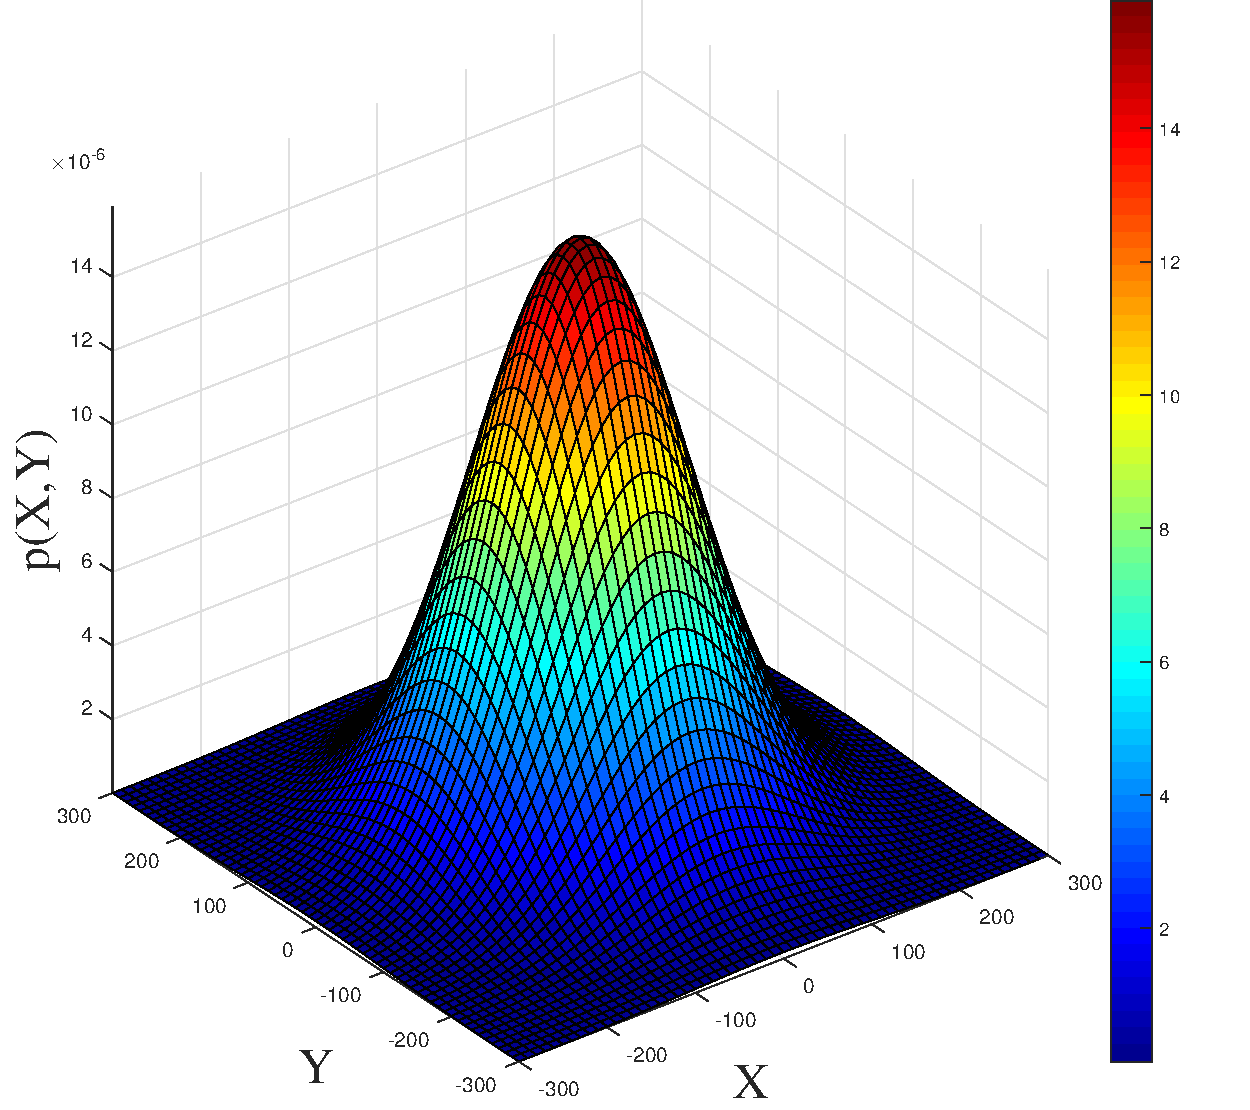
\includegraphics[width=4.5in]{imgs/1}
\caption{imgs/1}
\label{imgs/1}
\end{figure}

\begin{figure}[t]
\centering
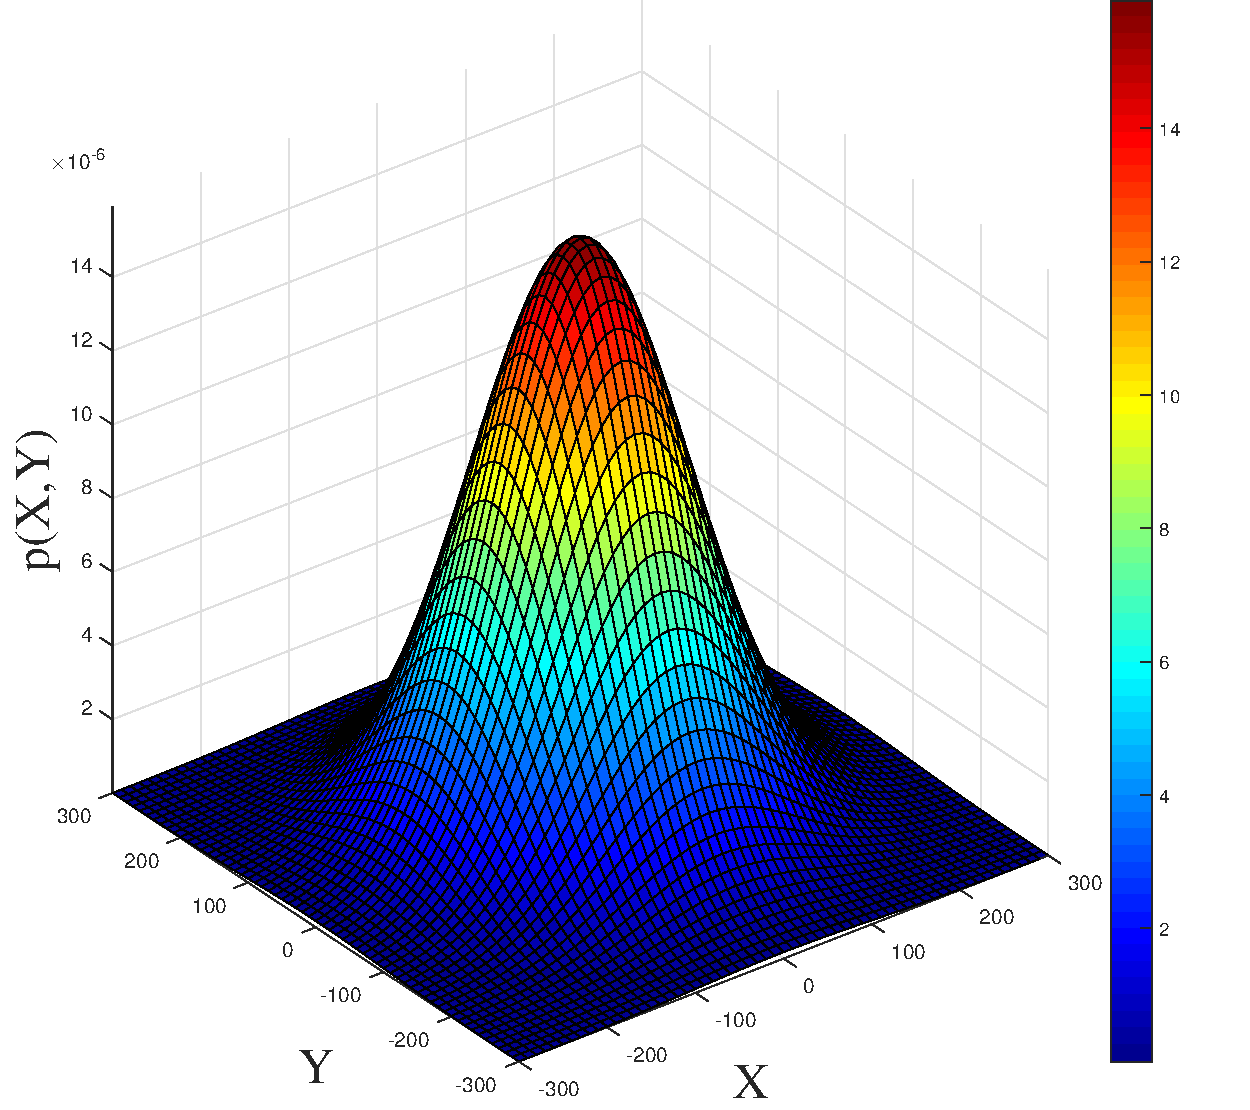
\includegraphics[width=4in]{imgs/1}
\caption{imgs/2.}
\label{imgs/2}
\end{figure}

The university was formed in 1963 as a federation of three existing colleges. The first of these, New Asia College, was established in 1949 by anti-Communist Confucian scholars from Mainland China amid the revolution there. Among the founders were Ch'ien Mu, Tang Junyi, and Tchang Pi-kai. Curriculum focused particularly on Chinese heritage and social concerns. The early years of this school were tumultuous, with the campus relocating several times between rented premises around Kowloon. Academics there were often self-exiled from the mainland and they struggled financially, with students sometimes sleeping on rooftops and teachers foregoing pay to sustain the college. Funds were gradually raised and the school moved to a new campus in Kau Pui Lung, built with the support of the Ford Foundation, in 1956.

\subsection{Origins--2}
The university was formed in 1963 as a federation of three existing colleges. The first of these, New Asia College, was established in 1949 by anti-Communist Confucian scholars from Mainland China amid the revolution there. Among the founders were Ch'ien Mu, Tang Junyi, and Tchang Pi-kai. Curriculum focused particularly on Chinese heritage and social concerns. The early years of this school were tumultuous, with the campus relocating several times between rented premises around Kowloon. Academics there were often self-exiled from the mainland and they struggled financially, with students sometimes sleeping on rooftops and teachers foregoing pay to sustain the college. Funds were gradually raised and the school moved to a new campus in Kau Pui Lung, built with the support of the Ford Foundation, in 1956.

The university was formed in 1963 as a federation of three existing colleges. The first of these, New Asia College, was established in 1949 by anti-Communist Confucian scholars from Mainland China amid the revolution there. Among the founders were Ch'ien Mu, Tang Junyi, and Tchang Pi-kai. Curriculum focused particularly on Chinese heritage and social concerns. The early years of this school were tumultuous, with the campus relocating several times between rented premises around Kowloon. Academics there were often self-exiled from the mainland and they struggled financially, with students sometimes sleeping on rooftops and teachers foregoing pay to sustain the college. Funds were gradually raised and the school moved to a new campus in Kau Pui Lung, built with the support of the Ford Foundation, in 1956.

\begin{figure}[t]
\centering
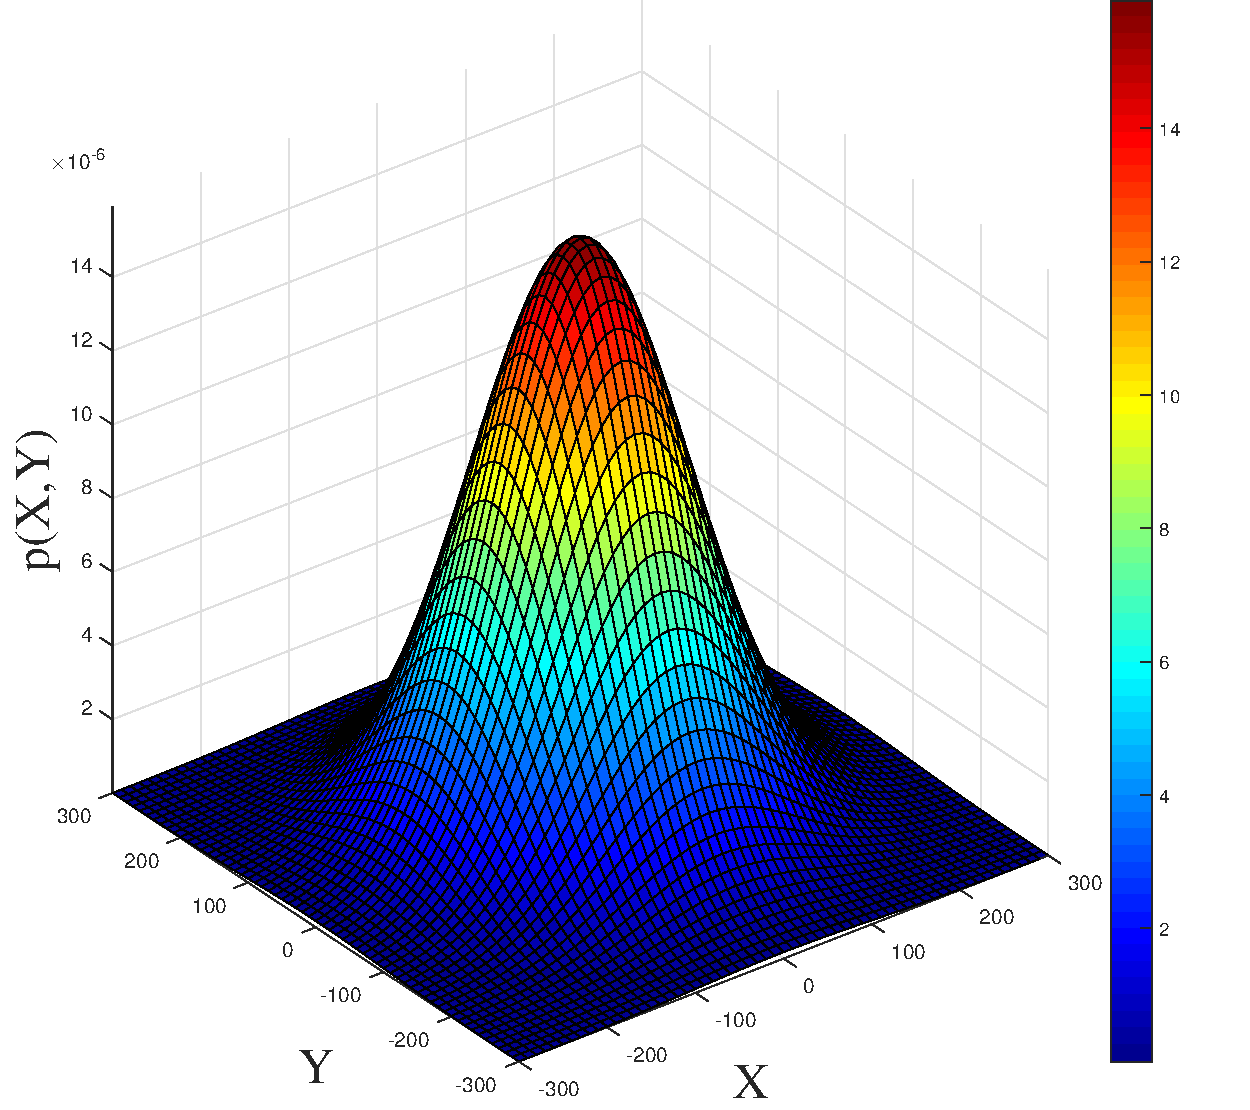
\includegraphics[width=5.5in]{imgs/1}
\caption{imgs/3.}
\label{imgs/3}
\end{figure}

The university was formed in 1963 as a federation of three existing colleges. The first of these, New Asia College, was established in 1949 by anti-Communist Confucian scholars from Mainland China amid the revolution there. Among the founders were Ch'ien Mu, Tang Junyi, and Tchang Pi-kai. Curriculum focused particularly on Chinese heritage and social concerns. The early years of this school were tumultuous, with the campus relocating several times between rented premises around Kowloon. Academics there were often self-exiled from the mainland and they struggled financially, with students sometimes sleeping on rooftops and teachers foregoing pay to sustain the college. Funds were gradually raised and the school moved to a new campus in Kau Pui Lung, built with the support of the Ford Foundation, in 1956.

The university was formed in 1963 as a federation of three existing colleges. The first of these, New Asia College, was established in 1949 by anti-Communist Confucian scholars from Mainland China amid the revolution there. Among the founders were Ch'ien Mu, Tang Junyi, and Tchang Pi-kai. Curriculum focused particularly on Chinese heritage and social concerns. The early years of this school were tumultuous, with the campus relocating several times between rented premises around Kowloon. Academics there were often self-exiled from the mainland and they struggled financially, with students sometimes sleeping on rooftops and teachers foregoing pay to sustain the college. Funds were gradually raised and the school moved to a new campus in Kau Pui Lung, built with the support of the Ford Foundation, in 1956.

The university was formed in 1963 as a federation of three existing colleges. The first of these, New Asia College, was established in 1949 by anti-Communist Confucian scholars from Mainland China amid the revolution there. Among the founders were Ch'ien Mu, Tang Junyi, and Tchang Pi-kai. Curriculum focused particularly on Chinese heritage and social concerns. The early years of this school were tumultuous, with the campus relocating several times between rented premises around Kowloon. Academics there were often self-exiled from the mainland and they struggled financially, with students sometimes sleeping on rooftops and teachers foregoing pay to sustain the college. Funds were gradually raised and the school moved to a new campus in Kau Pui Lung, built with the support of the Ford Foundation\cite{sadri2011logic}, in 1956\cite{sadri2011logic}.
\cite{sadri2011logic}proposed in \cite{heinze2004modelling}

\section{Foundation}
\subsection{Foundation--1}
The university was formed in 1963 as a federation of three existing colleges. The first of these, New Asia College, was established in 1949 by anti-Communist Confucian scholars from Mainland China amid the revolution there. Among the founders were Ch'ien Mu, Tang Junyi, and Tchang Pi-kai. Curriculum focused particularly on Chinese heritage and social concerns. The early years of this school were tumultuous, with the campus relocating several times between rented premises around Kowloon. Academics there were often self-exiled from the mainland and they struggled financially, with students sometimes sleeping on rooftops and teachers foregoing pay to sustain the college. Funds were gradually raised and the school moved to a new campus in Kau Pui Lung, built with the support of the Ford Foundation, in 1956.
\begin{table}[t]
	\caption{Table:1}
	\label{Table:1}       % Give a unique label
	\centering
	\begin{tabular}{ccccc}
		\hline\noalign{\smallskip}
		AS1 & AS2 &AS3  \\
		\noalign{\smallskip}\hline\noalign{\smallskip}
		1 & High 2	& 3\\
		\noalign{\smallskip}\hline
	\end{tabular}
\end{table}
\subsection{Foundation--2}
The university was formed in 1963 as a federation of three existing colleges. The first of these, New Asia College, was established in 1949 by anti-Communist Confucian scholars from Mainland China amid the revolution there. Among the founders were Ch'ien Mu, Tang Junyi, and Tchang Pi-kai. Curriculum focused particularly on Chinese heritage and social concerns. The early years of this school were tumultuous, with the campus relocating several times between rented premises around Kowloon. Academics there were often self-exiled from the mainland and they struggled financially, with students sometimes sleeping on rooftops and teachers foregoing pay to sustain the college. Funds were gradually raised and the school moved to a new campus in Kau Pui Lung, built with the support of the Ford Foundation, in 1956.

\begin{table}[t]
	\caption{Table:2}
	\label{Table:2}       % Give a unique label
	\centering
	\begin{tabular}{ccccc}
		\hline\noalign{\smallskip}
		AS1 & AS2 &AS3  \\
		\noalign{\smallskip}\hline\noalign{\smallskip}
		1 & High 2	& 3\\
		\noalign{\smallskip}\hline
	\end{tabular}
\end{table}

   % INCLUDE: introduction
% !TEX root = ../my-thesis.tex
%
\chapter{Conclusions and Future Work}
\label{sec:conclusion}
\cleanchapterquote{Stay hungry. Stay foolish.}{Steve Jobs}{(CEO of Apple Inc.)}

\noindent The university was formed in 1963 as a federation of three existing colleges. The first of these, New Asia College, was established in 1949 by anti-Communist Confucian scholars from Mainland China amid the revolution there. Among the founders were Ch'ien Mu, Tang Junyi, and Tchang Pi-kai. Curriculum focused particularly on Chinese heritage and social concerns. The early years of this school were tumultuous, with the campus relocating several times between rented premises around Kowloon. Academics there were often self-exiled from the mainland and they struggled financially, with students sometimes sleeping on rooftops and teachers foregoing pay to sustain the college. Funds were gradually raised and the school moved to a new campus in Kau Pui Lung, built with the support of the Ford Foundation, in 1956.

\section{Conclusions}
\subsection{Conclusions--1}
\noindent The university was formed in 1963 as a federation of three existing colleges. The first of these, New Asia College, was established in 1949 by anti-Communist Confucian scholars from Mainland China amid the revolution there. Among the founders were Ch'ien Mu, Tang Junyi, and Tchang Pi-kai. Curriculum focused particularly on Chinese heritage and social concerns. The early years of this school were tumultuous, with the campus relocating several times between rented premises around Kowloon. Academics there were often self-exiled from the mainland and they struggled financially, with students sometimes sleeping on rooftops and teachers foregoing pay to sustain the college. Funds were gradually raised and the school moved to a new campus in Kau Pui Lung, built with the support of the Ford Foundation, in 1956.


The university was formed in 1963 as a federation of three existing colleges. The first of these, New Asia College, was established in 1949 by anti-Communist Confucian scholars from Mainland China amid the revolution there. Among the founders were Ch'ien Mu, Tang Junyi, and Tchang Pi-kai. Curriculum focused particularly on Chinese heritage and social concerns. The early years of this school were tumultuous, with the campus relocating several times between rented premises around Kowloon. Academics there were often self-exiled from the mainland and they struggled financially, with students sometimes sleeping on rooftops and teachers foregoing pay to sustain the college. Funds were gradually raised and the school moved to a new campus in Kau Pui Lung, built with the support of the Ford Foundation, in 1956.

\subsection{Conclusions--2}
The university was formed in 1963 as a federation of three existing colleges. The first of these, New Asia College, was established in 1949 by anti-Communist Confucian scholars from Mainland China amid the revolution there. Among the founders were Ch'ien Mu, Tang Junyi, and Tchang Pi-kai. Curriculum focused particularly on Chinese heritage and social concerns. The early years of this school were tumultuous, with the campus relocating several times between rented premises around Kowloon. Academics there were often self-exiled from the mainland and they struggled financially, with students sometimes sleeping on rooftops and teachers foregoing pay to sustain the college. Funds were gradually raised and the school moved to a new campus in Kau Pui Lung, built with the support of the Ford Foundation, in 1956.

The university was formed in 1963 as a federation of three existing colleges. The first of these, New Asia College, was established in 1949 by anti-Communist Confucian scholars from Mainland China amid the revolution there. Among the founders were Ch'ien Mu, Tang Junyi, and Tchang Pi-kai. Curriculum focused particularly on Chinese heritage and social concerns. The early years of this school were tumultuous, with the campus relocating several times between rented premises around Kowloon. Academics there were often self-exiled from the mainland and they struggled financially, with students sometimes sleeping on rooftops and teachers foregoing pay to sustain the college. Funds were gradually raised and the school moved to a new campus in Kau Pui Lung, built with the support of the Ford Foundation, in 1956.


The university was formed in 1963 as a federation of three existing colleges. The first of these, New Asia College, was established in 1949 by anti-Communist Confucian scholars from Mainland China amid the revolution there. Among the founders were Ch'ien Mu, Tang Junyi, and Tchang Pi-kai. Curriculum focused particularly on Chinese heritage and social concerns. The early years of this school were tumultuous, with the campus relocating several times between rented premises around Kowloon. Academics there were often self-exiled from the mainland and they struggled financially, with students sometimes sleeping on rooftops and teachers foregoing pay to sustain the college. Funds were gradually raised and the school moved to a new campus in Kau Pui Lung, built with the support of the Ford Foundation, in 1956.

The university was formed in 1963 as a federation of three existing colleges. The first of these, New Asia College, was established in 1949 by anti-Communist Confucian scholars from Mainland China amid the revolution there. Among the founders were Ch'ien Mu, Tang Junyi, and Tchang Pi-kai. Curriculum focused particularly on Chinese heritage and social concerns. The early years of this school were tumultuous, with the campus relocating several times between rented premises around Kowloon. Academics there were often self-exiled from the mainland and they struggled financially, with students sometimes sleeping on rooftops and teachers foregoing pay to sustain the college. Funds were gradually raised and the school moved to a new campus in Kau Pui Lung, built with the support of the Ford Foundation, in 1956.

The university was formed in 1963 as a federation of three existing colleges. The first of these, New Asia College, was established in 1949 by anti-Communist Confucian scholars from Mainland China amid the revolution there. Among the founders were Ch'ien Mu, Tang Junyi, and Tchang Pi-kai. Curriculum focused particularly on Chinese heritage and social concerns. The early years of this school were tumultuous, with the campus relocating several times between rented premises around Kowloon. Academics there were often self-exiled from the mainland and they struggled financially, with students sometimes sleeping on rooftops and teachers foregoing pay to sustain the college. Funds were gradually raised and the school moved to a new campus in Kau Pui Lung, built with the support of the Ford Foundation, in 1956.


\section{Future Work}
\subsection{Future Work--1}
The university was formed in 1963 as a federation of three existing colleges. The first of these, New Asia College, was established in 1949 by anti-Communist Confucian scholars from Mainland China amid the revolution there. Among the founders were Ch'ien Mu, Tang Junyi, and Tchang Pi-kai. Curriculum focused particularly on Chinese heritage and social concerns. The early years of this school were tumultuous, with the campus relocating several times between rented premises around Kowloon. Academics there were often self-exiled from the mainland and they struggled financially, with students sometimes sleeping on rooftops and teachers foregoing pay to sustain the college. Funds were gradually raised and the school moved to a new campus in Kau Pui Lung, built with the support of the Ford Foundation, in 1956.
\subsection{Future Work--2}
The university was formed in 1963 as a federation of three existing colleges. The first of these, New Asia College, was established in 1949 by anti-Communist Confucian scholars from Mainland China amid the revolution there. Among the founders were Ch'ien Mu, Tang Junyi, and Tchang Pi-kai. Curriculum focused particularly on Chinese heritage and social concerns. The early years of this school were tumultuous, with the campus relocating several times between rented premises around Kowloon. Academics there were often self-exiled from the mainland and they struggled financially, with students sometimes sleeping on rooftops and teachers foregoing pay to sustain the college. Funds were gradually raised and the school moved to a new campus in Kau Pui Lung, built with the support of the Ford Foundation, in 1956.     % INCLUDE: conclusion

% --------------------------
% Back matter
% --------------------------
\appendix\cleardoublepage

%
{%
\setstretch{1.5}
\renewcommand{\bibfont}{\normalfont\small}
\setlength{\biblabelsep}{0pt}
\setlength{\bibitemsep}{0.5\baselineskip plus 0.5\baselineskip}
\printbibliography%[nottype=online]
%\printbibliography[heading=subbibliography,title={Webpages},type=online,prefixnumbers={@}]
}
\cleardoublepage



\mbox{}

% **************************************************
% End of Document CONTENT
% **************************************************
\end{document}
